\section{Introduction}
\label{sec:introduction}

Research papers often say where a study falls short and what should be done next. Authors acknowledge the limitations of their own work, which tell readers how far its design, execution and interpretation limit the findings~\cite{kilicoglu2018automatic,lan2024automatic}. They propose future work that names the extensions and open questions they consider worth pursuing~\cite{zhu2019recognizing,zhang2023fws}, and they point to unsolved problems in their field when they motivate their own work. We call these statements \emph{author-stated research gaps}: limitations of the authors' own work, future-work directions they propose, and open problems they identify. Collected across many papers, they are a natural input for automated idea generation, because each one is a claim, made by a domain expert, about what is still missing.

Gap statements are hard to find for four reasons. They are rare: in the test sets we use, they make up 2.6\% of the sentences of randomized controlled trial (RCT) reports, 5.7\% of full arXiv and biomedical papers and 14.6\% of conclusion sections. They are scattered: a limitation may sit in a dedicated section, in the discussion or next to a methodological choice, and in computer-science papers many gaps appear in the methods and experiments sections. Many sentences look like gaps without being one, such as a criticism of prior work or a restated result. And the output must stay attributable: a system that writes plausible criticism answers a different question from one that finds what the authors actually wrote~\cite{xu2025llms,mishra2026tree}.

A large language model (LLM) can judge whether a sentence states a gap; the open question is how much of the paper to give it. Judging every sentence in a separate request is expensive. Giving the model the whole paper is simpler, but then a few relevant sentences sit among thousands to tens of thousands of tokens, and LLMs use information in the middle of long inputs less reliably~\cite{liu2024lost}, with accuracy falling as inputs grow~\cite{hsieh2024ruler}. This matters most for the smaller models that make processing large collections affordable.

Our idea is to shrink the LLM's job. Instead of asking it to find the gaps in a paper, we ask it only to verify a short list of candidates that cheaper components have already selected. Earlier extraction work points in the same direction: clinical limitation recognition uses section titles and limitation keywords to select candidate sentences, and these rules alone were more accurate than supervised classifiers~\cite{kilicoglu2018automatic}; future-work recognition separates locating sentences from grouping or classifying them~\cite{zhu2019recognizing,zhang2023fws}. We build this division of labour into a three-stage funnel (Figure~\ref{fig:pipeline-overview}). Stage~A removes text that is unlikely to contain gaps, Stage~B selects candidate sentences with a zero-shot natural-language-inference (NLI) classifier, and Stage~C asks an LLM to keep or drop each candidate. No stage rewrites text, so every output is a sentence the authors wrote. Stage~B needs no gap-labelled training data, so the same funnel runs on biomedical and computer-science papers. Because the LLM only verifies, its behaviour can also be steered with a single instruction: a mode paragraph in the system prompt sets Stage~C to high precision, balanced or high recall. A false gap wastes effort in idea generation, so precision is our primary goal and high precision is the main mode.

\begin{figure}[!htb]
\begin{adjustwidth}{-\extralength}{0cm}
\centering
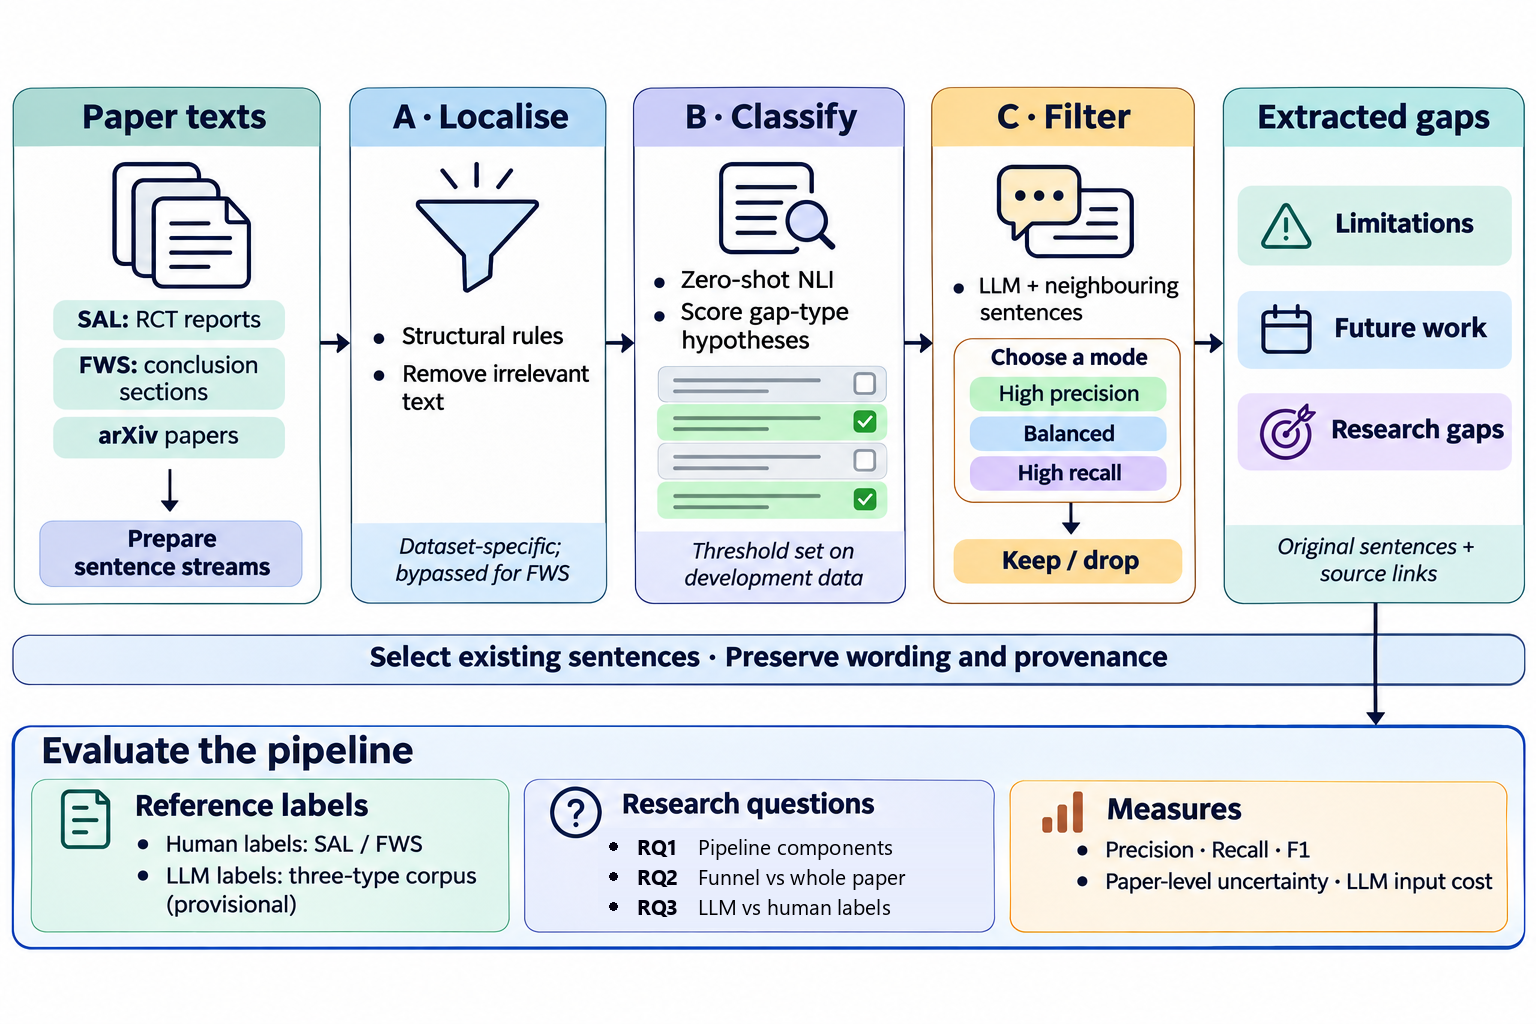
\includegraphics[width=\fulllength]{figures/gap2idea_graphical_abstract_v2.png}
\end{adjustwidth}
\caption{Overview of the funnel. Each paper is split into sentences. Stage~A removes text that is unlikely to contain gaps (its rules depend on the dataset; FWS skips it), Stage~B selects candidate sentences with a zero-shot NLI classifier, and Stage~C asks an LLM to keep or drop each candidate. The three filter modes are alternative instructions for Stage~C, not consecutive steps. Every output is an original sentence with its source. Evaluation uses human labels on SAL (limitations) and FWS (future work), and provisional LLM labels for all three gap types.\label{fig:pipeline-overview}}
\end{figure}

We evaluate the funnel on two benchmarks with human labels, self-acknowledged limitations in RCT reports (SAL)~\cite{lan2024automatic} and future-work sentences in natural language processing (NLP) papers (FWS)~\cite{zhang2023fws}. Each covers one gap type in one field, so we also built a corpus of 230 arXiv and biomedical papers in which two LLMs labelled all three gap types independently and an LLM judge resolved their disagreements. We compare the funnel with giving the same LLM the whole paper, using 27B, 9B and 4B models, and ask four questions:
\begin{itemize}
  \item \textbf{RQ1 (stages).} How much does each stage change precision and recall on full papers?
  \item \textbf{RQ2 (precision control).} Does one instruction set the precision--recall trade-off of the LLM filter consistently across datasets?
  \item \textbf{RQ3 (whole-paper prompting).} How does the funnel compare with giving the same LLM the whole paper, in accuracy and cost, and does the answer depend on the size of the LLM?
  \item \textbf{RQ4 (classifier).} Is a training-free classifier enough for Stage~B, compared with a classifier trained on human labels or one fine-tuned on our LLM labels?
\end{itemize}

Narrowing the LLM's job pays off most where the LLM is weakest. With a 4B model, whole-paper prompting kept most sentences of several long arXiv papers. The funnel, sending each paper's candidates in a single call with the Stage~B classifier fine-tuned on our LLM labels, raised $F_1$ on arXiv from 0.30 to 0.48 while the LLM read about seven times fewer input tokens (Tables~\ref{tab:wholecost} and~\ref{tab:variants}). With a 27B model, the two approaches are closer: the funnel scores higher on the human-labelled benchmarks with less input, and whole-paper prompting scores higher on arXiv papers, whose labels were themselves made from whole papers. Our contributions are:
\begin{enumerate}
  \item \textbf{A source-preserving funnel for gap extraction} in which the LLM only verifies candidates, every output is an author-written sentence, and one instruction sets the trade-off between precision and recall. The modes kept their order on every dataset; in high-precision mode, verification raised precision on SAL from 29.1\% to 66.2\% at 84.9\% recall (Sections~\ref{sec:rq1} and~\ref{sec:rq2}).
  \item \textbf{A comparison with whole-paper prompting across three LLM sizes}, in accuracy and cost. On full papers, the funnel reads about 7--8 times fewer input tokens in its one-call-per-paper format, and its advantage grows as the model gets smaller (Sections~\ref{sec:rq3} and~\ref{sec:format}).
  \item \textbf{An analysis of the stages and of the classifier.} Stage~A helps where section headings are informative, Stage~B sets the recall ceiling because Stage~C can only remove candidates, and Stage~C supplies most of the precision gain on full papers. A zero-shot classifier comes within 0.021 $F_1$ of a supervised one on SAL, at lower precision (Section~\ref{sec:rq4}).
  \item \textbf{A three-type evaluation corpus and two evaluation pitfalls.} We release the LLM-labelled corpus with every LLM verdict behind our results. We also show that the same SAL output has 66.2\% precision against human labels and 93.2\% against LLM labels, and that letter case reveals the label in the public FWS corpus, so we lowercase all FWS text (Sections~\ref{sec:label-source} and~\ref{sec:fws-case}).
\end{enumerate}

The scope of this paper is extraction. Whether an extracted gap is still open, and whether it leads to a useful research idea, are separate questions. Section~\ref{sec:related} reviews related work. Section~\ref{sec:methods} describes the data, the funnel and the comparisons. Section~\ref{sec:results} reports the results, Section~\ref{sec:discussion} discusses them and the limitations of the study, and Section~\ref{sec:conclusions} concludes.
